

\documentclass[a4paper, 11pt]{article} 



\usepackage{graphicx} 

\usepackage[parfill]{parskip} % Activate to begin paragraphs with an empty line rather than an indent

%%% PACKAGES
\usepackage{booktabs} % for much better looking tables
\usepackage{array} % for better arrays (eg matrices) in maths
\usepackage{paralist} % very flexible & customisable lists (eg. enumerate/itemize, etc.)
\usepackage{verbatim} % adds environment for commenting out blocks of text & for better verbatim
\usepackage[utf8, latin1]{inputenc} 
\usepackage{subfig} % make it possible to include more than one captioned figure/table in a single float
\usepackage{lscape} %turn landscape
\usepackage{amsmath} %math formatting
\usepackage{bbold} %math formatting
\usepackage[colorlinks, citecolor=blue]{hyperref}

%formatting allows footnotes to keep black color
\makeatletter
\def\@footnotecolor{red}
\define@key{Hyp}{footnotecolor}{%
	\HyColor@HyperrefColor{#1}\@footnotecolor%
}
\def\@footnotemark{%
	\leavevmode
	\ifhmode\edef\@x@sf{\the\spacefactor}\nobreak\fi
	\stepcounter{Hfootnote}%
	\global\let\Hy@saved@currentHref\@currentHref
	\hyper@makecurrent{Hfootnote}%
	\global\let\Hy@footnote@currentHref\@currentHref
	\global\let\@currentHref\Hy@saved@currentHref
	\hyper@linkstart{footnote}{\Hy@footnote@currentHref}%
	\@makefnmark
	\hyper@linkend
	\ifhmode\spacefactor\@x@sf\fi
	\relax
}%
\makeatother
\hypersetup{footnotecolor=black}

\renewcommand{\thesection}{\Alph{section}.}

\title{EDLD 650: Data Analysis and Replication Exercise (DARE) 2}
\author{David D. Liebowitz}
\date{Due: Feb. 5, 2024} 

\begin{document}
\maketitle



\section{Assumption tests (4 points)}

\begin{enumerate}
	\item[A1.] Our identification strategy relies on the fact that California elementary schools in the bottom two deciles of performance received supplemental funding for instructional materials as a result of the Williams settlement. For our regression discontinuity approach to be successful, schools' API score (our \textit{forcing variable}) must predict differences in the probability that schools actually receive additional funding. \autoref{fig:force} plots the probability of receipt of this funding in 2005 by 2003 API score, centered at the elementary school API cutoff score (643). In Panel A, we present all schools and in Panel B we aggregate schools in bins of 3 API scores for visual clarity. In both instances, our forcing variable (API score) is a strong (in fact, nearly perfect) predictor of receipt of Williams funding. 

\begin{figure} 
\begin{center}
\subfloat[Discrete API values]{
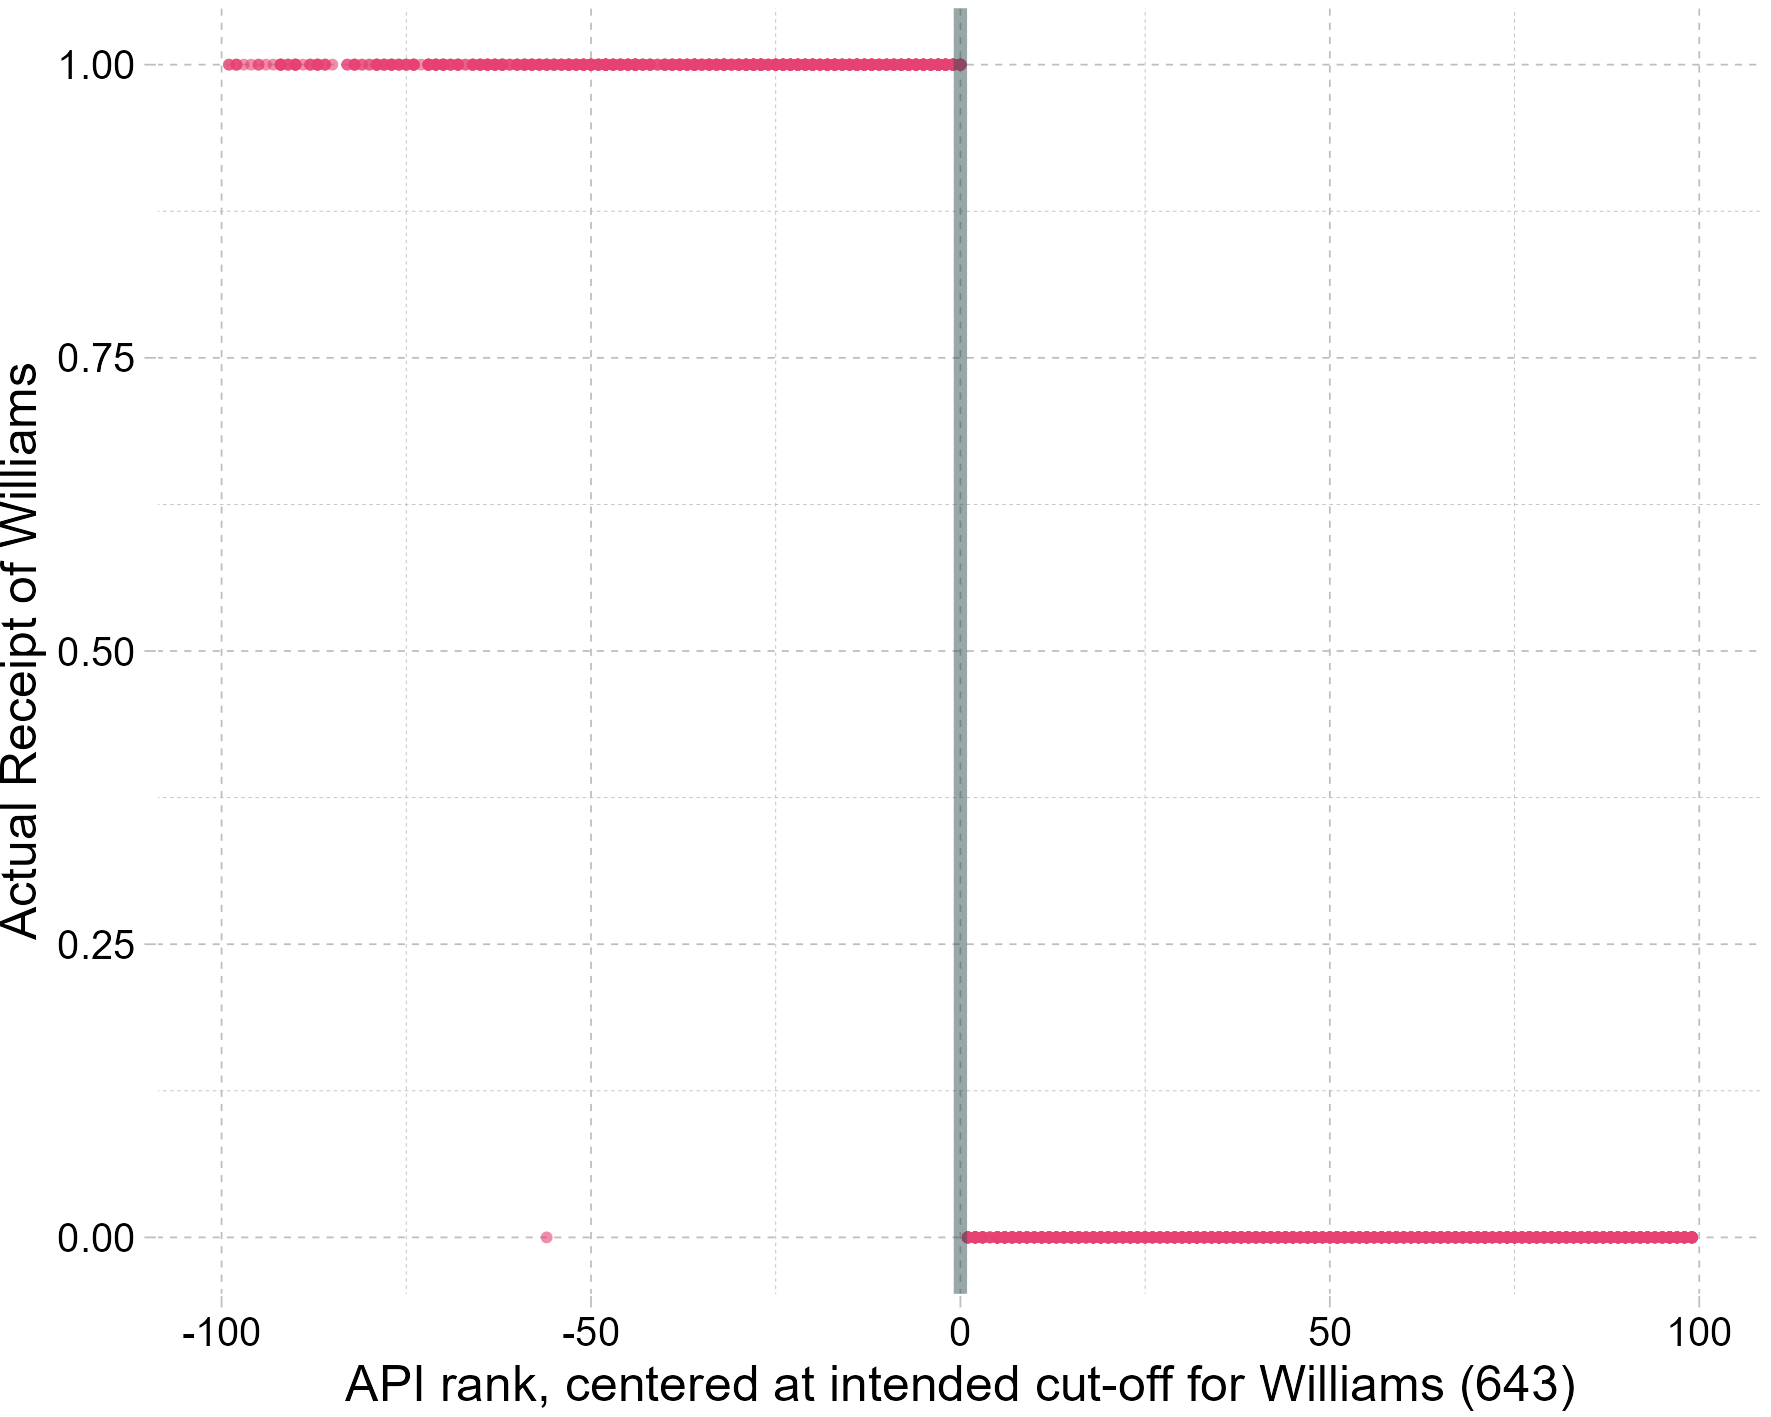
\includegraphics[scale=0.4]{figures/williams_treat.png}
}
\subfloat[Binned API values]{
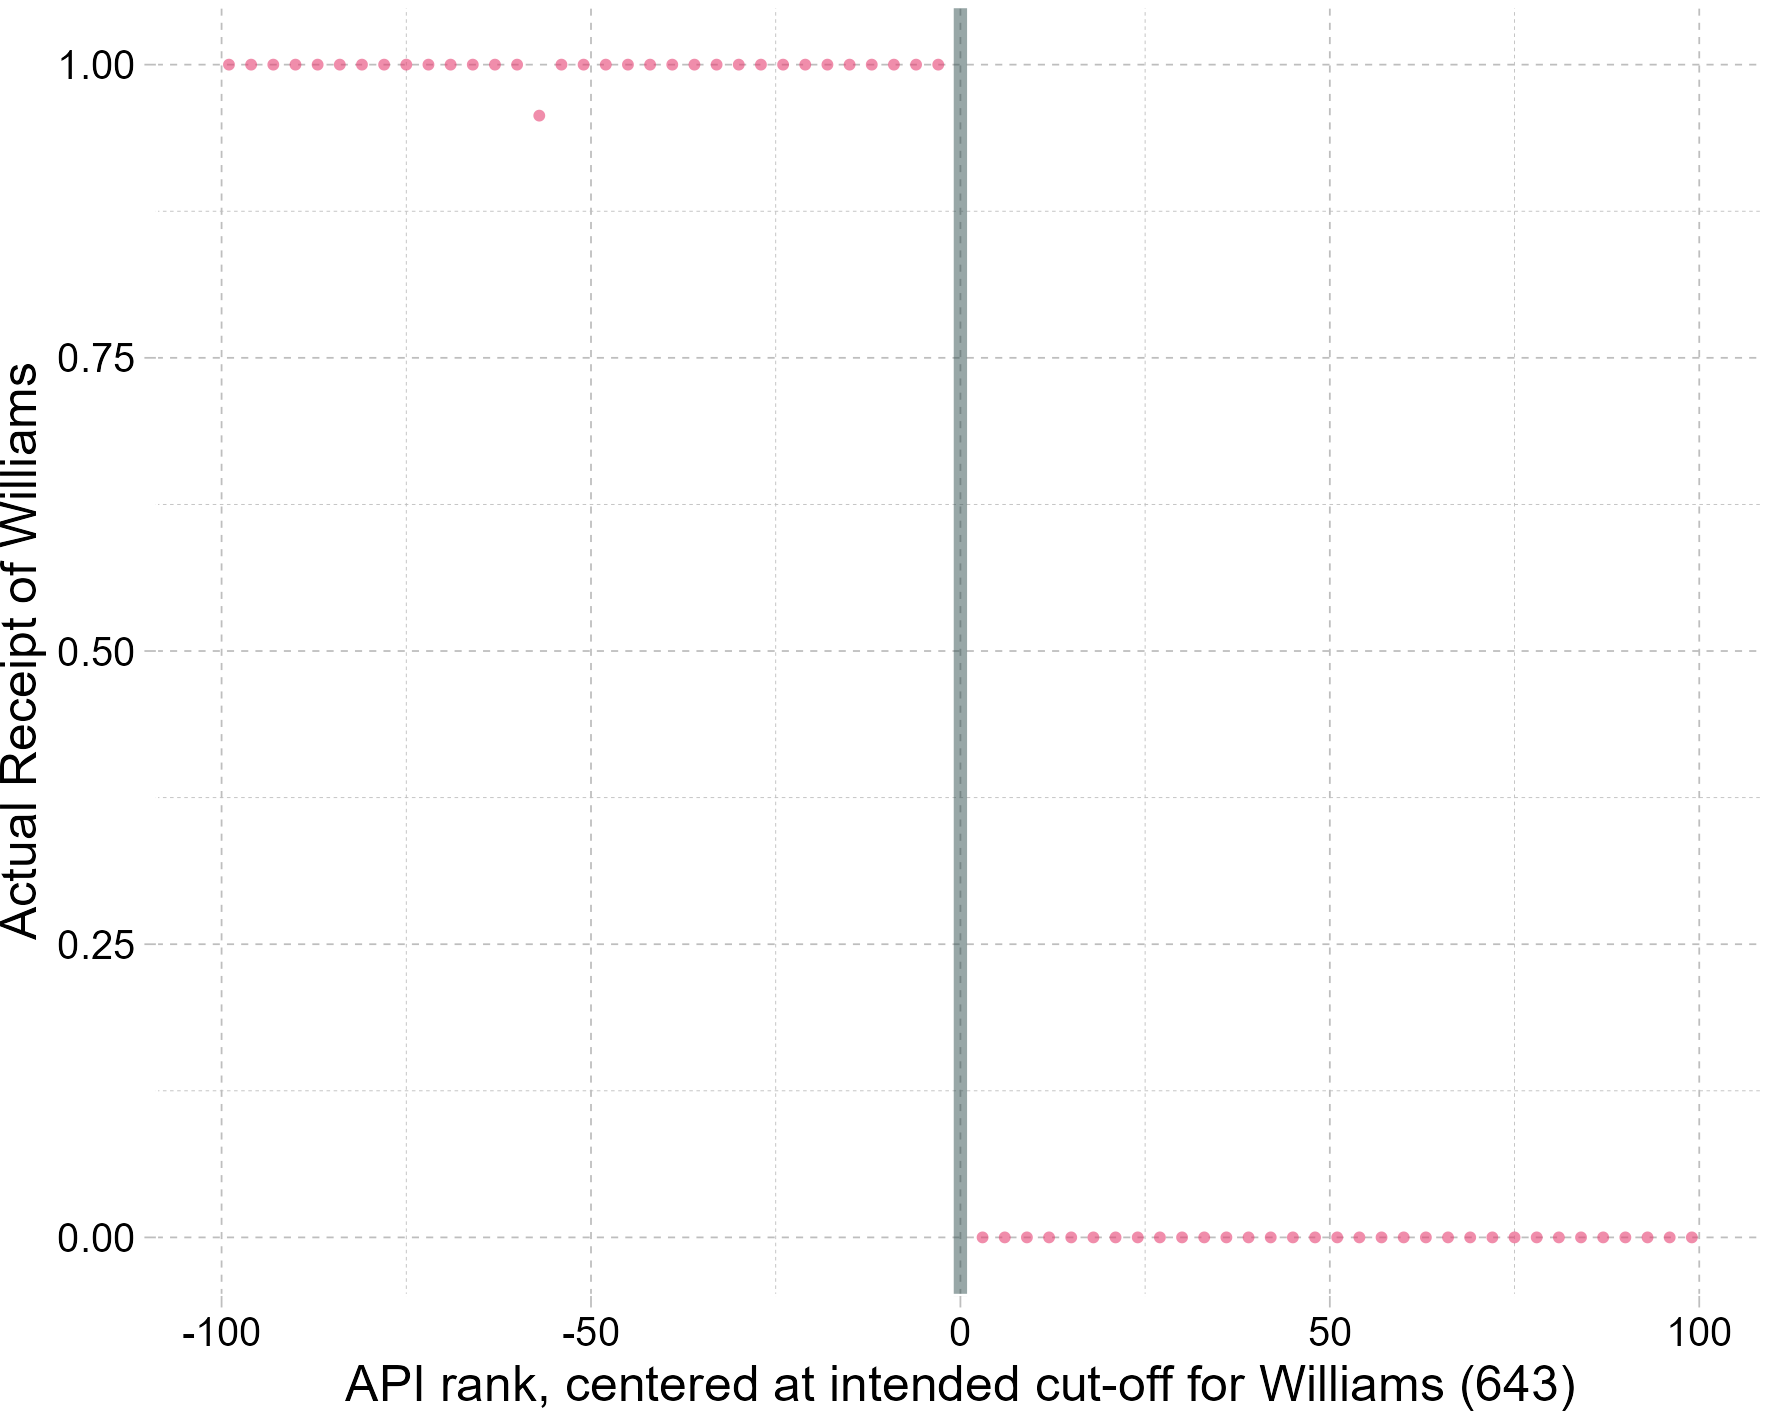
\includegraphics[scale=0.4]{figures/williams_treat_bin.png}
}
\caption{Probability of receipt of Williams funding by centered API score}
\label{fig:force}
\end{center}
\end{figure}

	\item[A2.] Our modeling approach depends on our ability to project a smooth relationship between API score and student test scores, that units (schools) did not manipulate their position around the discontinuity in textbook funding and that schools immediately on one side of the discontinuity were not observably different than schools on the other side. In \autoref{fig:bunch}, we present evidence that there is no evident bunching of schools just to the left of the discontinuous award of textbook funding. While there are slightly more schools with API scores that just qualify them for additional funding, the discrepancy is similar to other random variation throughout the distribution of $\pm$100 API scores. Thus, we are fairly confident that bunching does not threaten our assumptions.

	In \autoref{fig:manip}, we address the possibility that schools that received Williams funding might not have been equal in expectation to those that did not. While we can never fully address the possibility that unobservable attributes vary around the discontinuity, we observe no discontinuous jump in the proportion of students eligible for free- and reduced-price lunch. This provides suggestive evidence that no sorting occurred. Note that we display school characteristics for the 2002-03 school year (prior to determination of Williams eligibility). School characteristics post-cut score determination are endogenous to the receipt of funding and are therefore not valid tests for the presence of sorting.

\begin{figure} 
\begin{center}
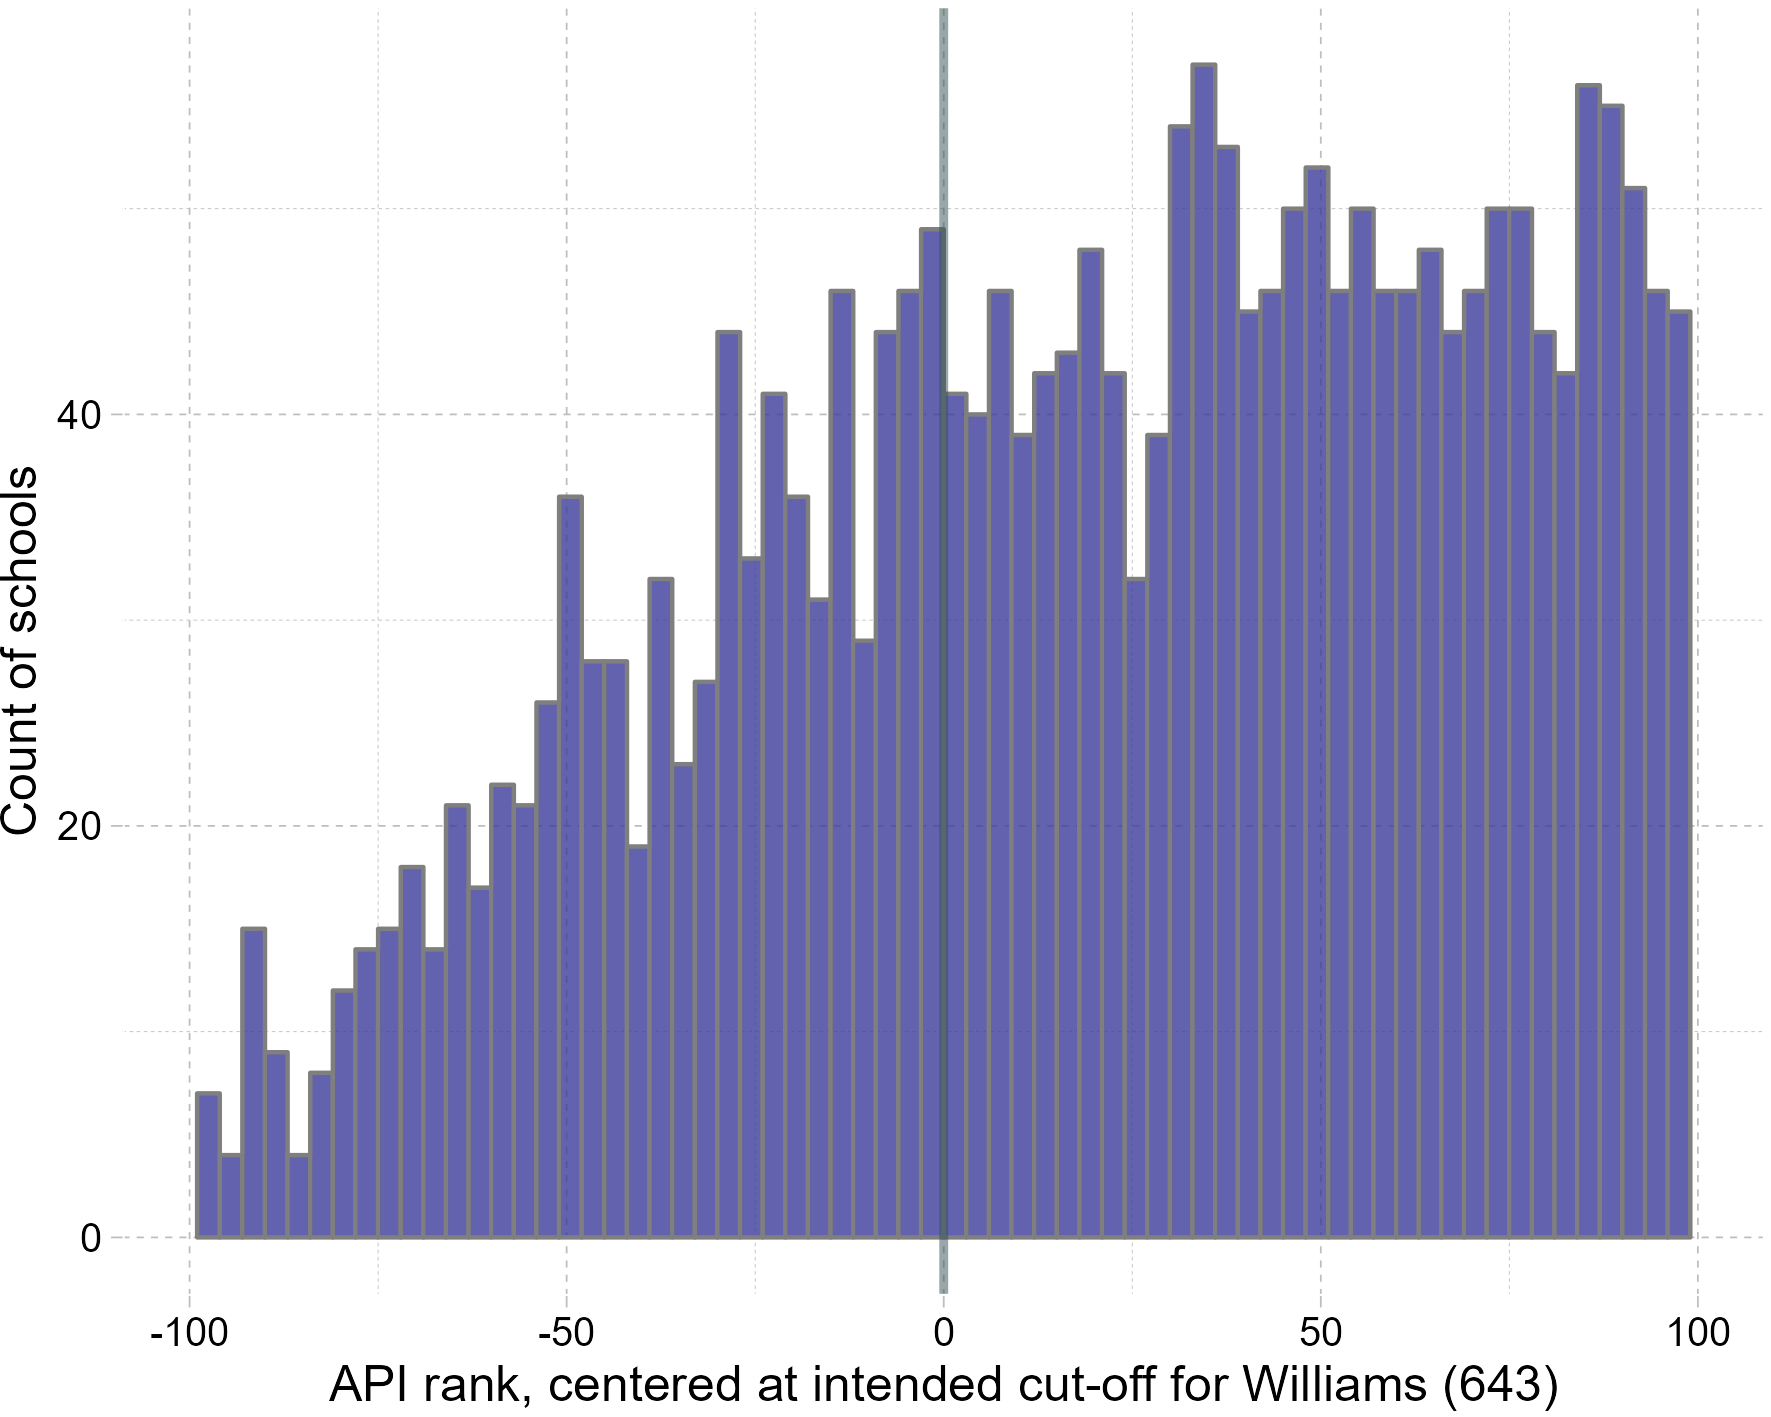
\includegraphics[scale=0.8]{figures/williams_bunch.png}
\caption{Count of schools by centered API score}
\label{fig:bunch}
\end{center}
\end{figure}

\begin{figure} 
\begin{center}
\subfloat[Best fit at median quantile]{
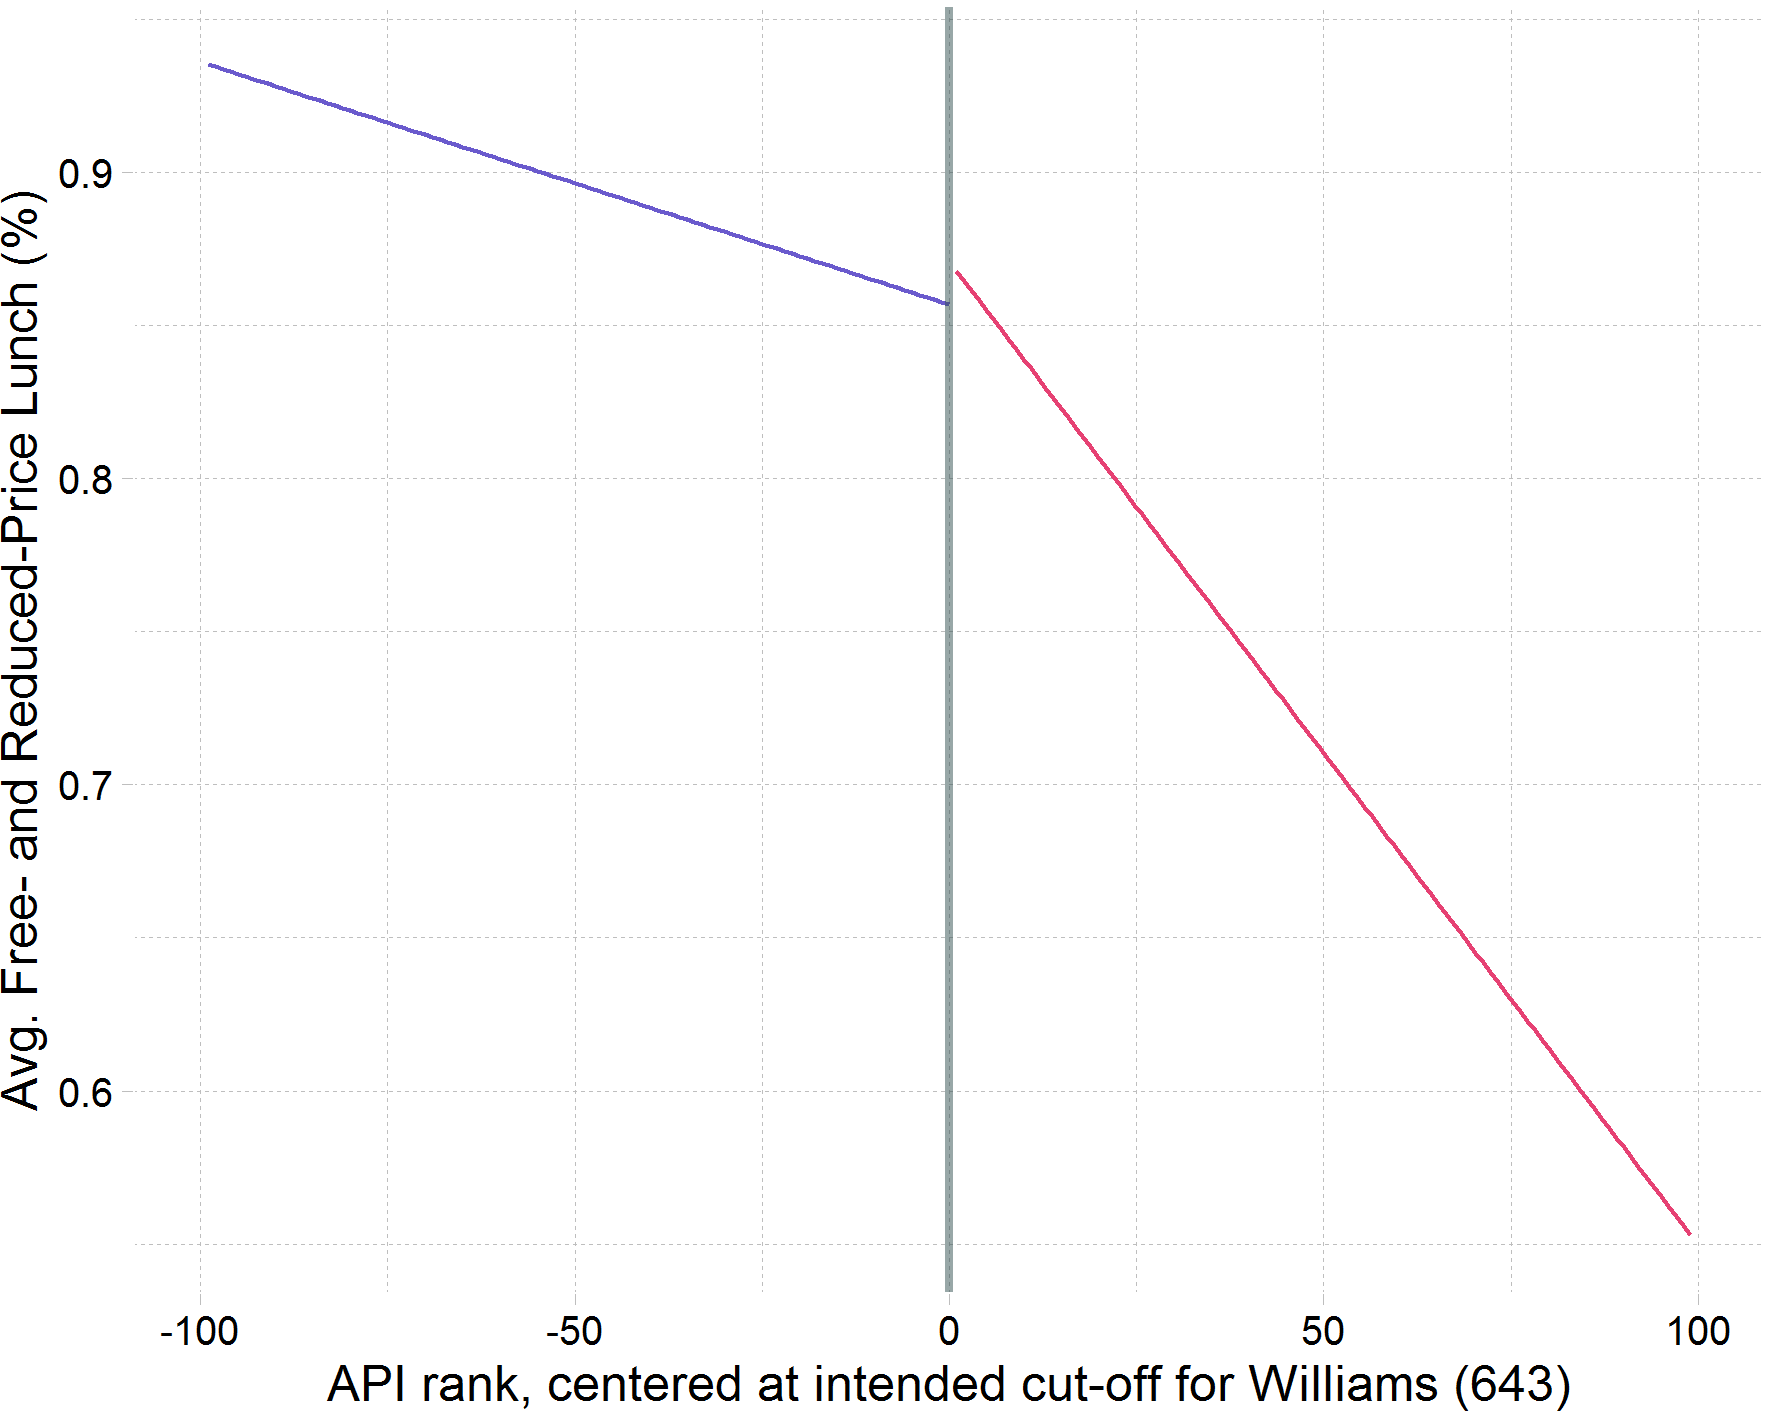
\includegraphics[scale=0.4]{figures/williams_sort.png}
}
\subfloat[Binned API values]{
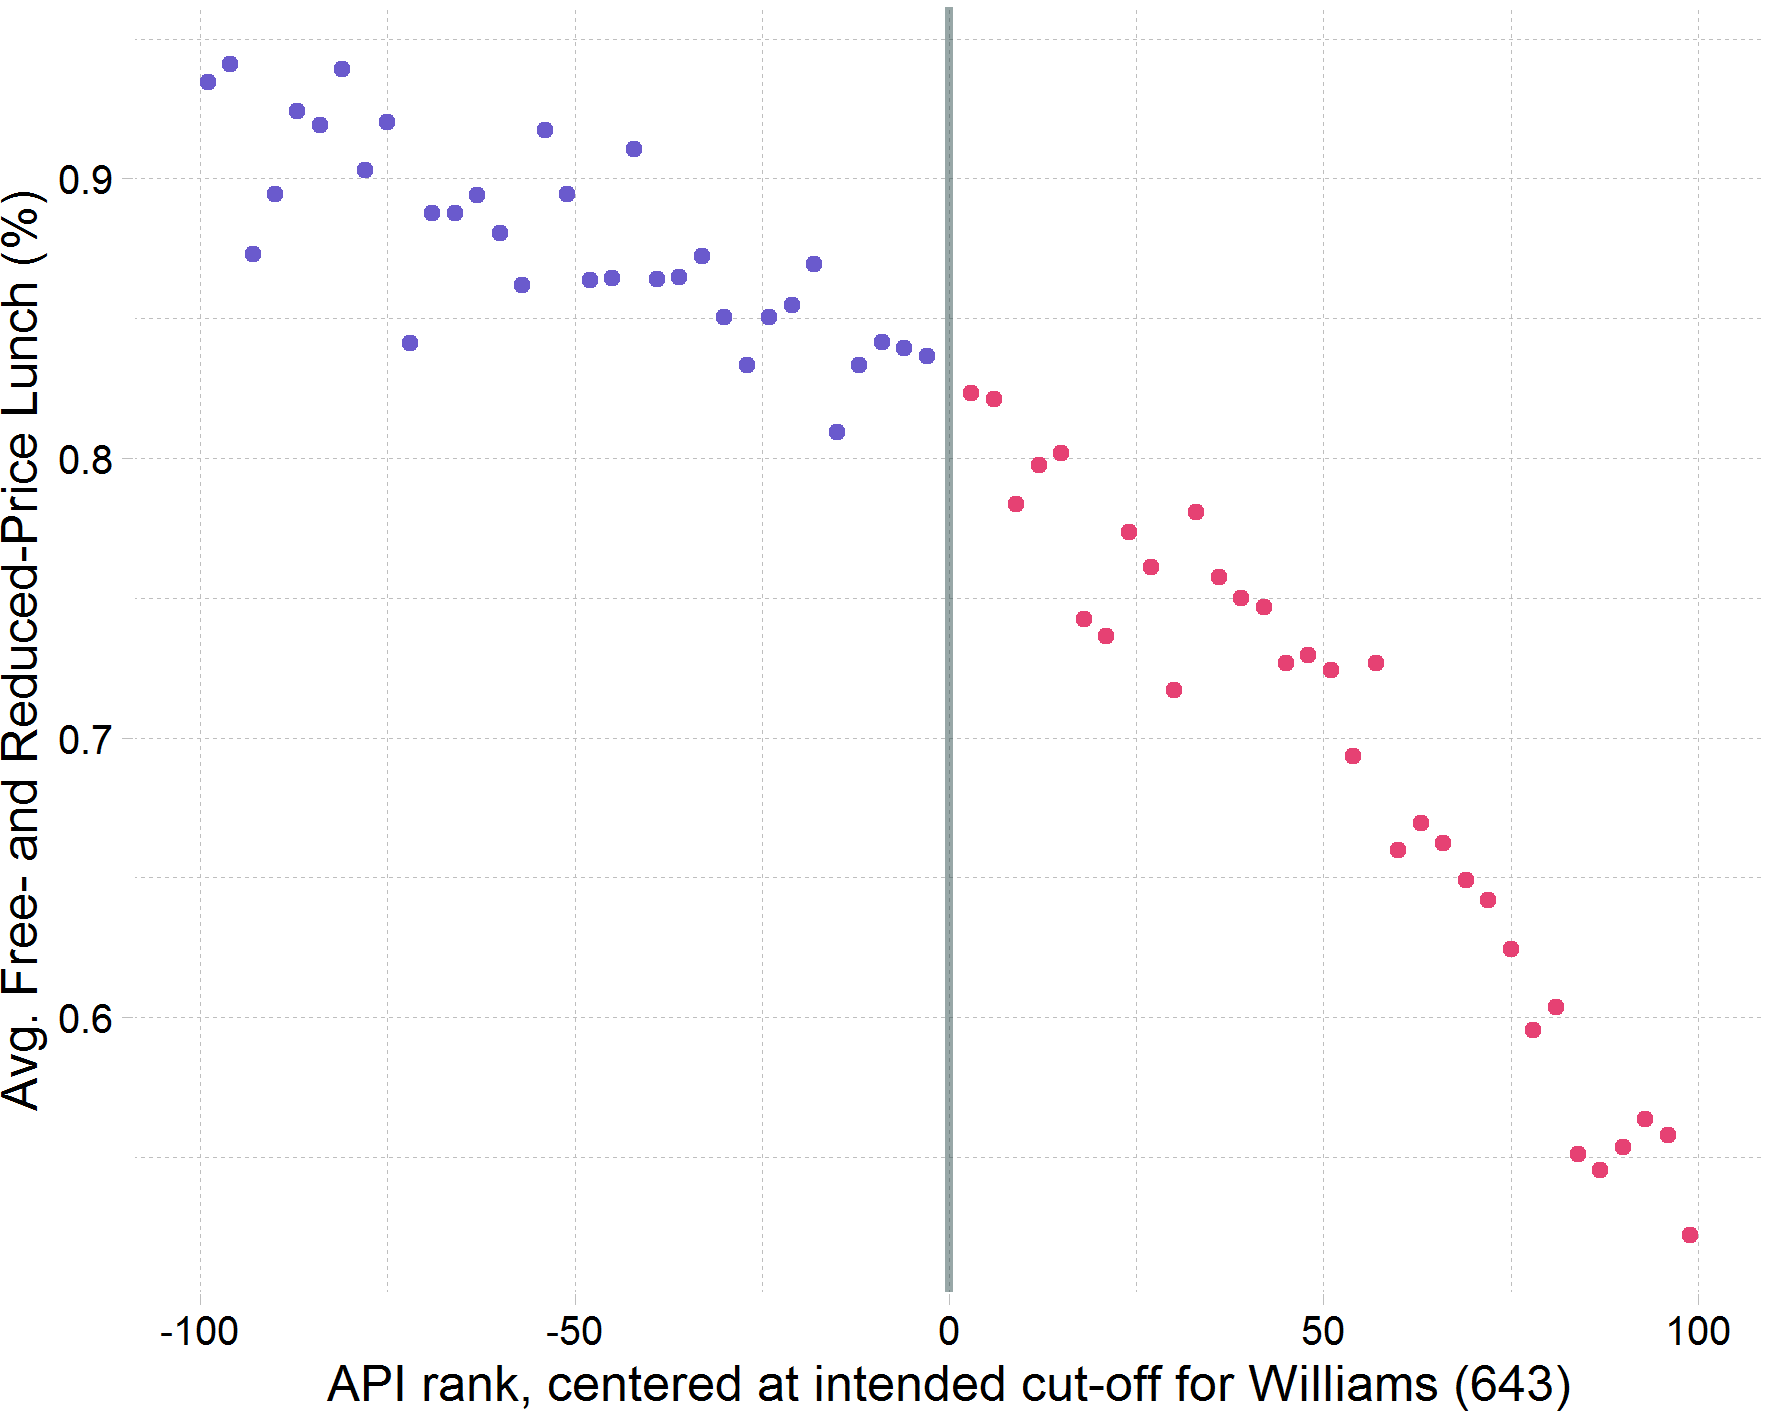
\includegraphics[scale=0.4]{figures/williams_bin_sort.png}
}
\caption{Free- and reduced-price lunch proportion by centered API score}
\label{fig:manip}
\end{center}
\end{figure}

	\item[A3.] \textbf{\textit{Optional Extension}} In \autoref{tab:descriptives}, we present descriptive statistics on our analytic sample of 16,462 elementary schools. These low-performing elementary schools educate disproportionately Hispanic students from low-income backgrounds.\footnote{We use the term ``Hispanic or Latino'' (rather than Latino/a, Latinx or other nomenclature) because this is the federally recognized term used by the Office of Management and Budget/Census Bureau with which ethnicity data are harmonized at sub-national levels in the United States.} 

	In comparison to the full set of K-12 schools in the original Holden dataset, these schools are slightly smaller and have lower test score and API rank values. This is entirely a function of the fact that elementary schools are generally smaller in size and that their test and API scores are on a different scale. These differences, therefore, do not concern us. Elementary schools in California appear to be disproportionately Hispanic/Latino and poor, compared to middle and high schools. Pupil-teacher ratios are, surprisingly, only marginally smaller in elementary schools than in the full sample (around 20:1 for elementary compared to 21:1 for all schools).


% Table created by stargazer v.5.2.2 by Marek Hlavac, Harvard University. E-mail: hlavac at fas.harvard.edu
% Date and time: Wed, Jan 05, 2022 - 1:00:32 PM
\begin{table}[!htbp] \centering 
  \caption{Descriptive Statistics} 
  \label{} 
\begin{tabular}{@{\extracolsep{5pt}}lccc} 
\\[-1.8ex]\hline 
\hline \\[-1.8ex] 
Statistic & \multicolumn{1}{c}{N} & \multicolumn{1}{c}{Mean} & \multicolumn{1}{c}{St. Dev.} \\ 
\hline \\[-1.8ex] 
Mean State-Year Enrollment & 470 & 21,897 & 4,622 \\ 
Mean Yearly Enrollment & 470 & 881,631 & 232,717 \\ 
Pct. low-income & 470 & 0.55 & 0.05 \\ 
Pct. American Indian/Native AK & 470 & 0.01 & 0.001 \\ 
Pct. Asian/Pacific-Islander & 470 & 0.05 & 0.01 \\ 
Pct. Black & 470 & 0.13 & 0.02 \\ 
Pct. White Non-Hispanic & 470 & 0.55 & 0.02 \\ 
Pct. Hispanic & 470 & 0.19 & 0.05 \\ 
Pct. States by year Implementing PBIS & 341 & 0.72 & 0.45 \\ 
Daily Referalls per 500 students - Classroom & 470 & 1.39 & 0.14 \\ 
Daily Referalls per 500 students - Other & 470 & 1.33 & 0.13 \\ 
Daily Referalls per 500 students - Subjective & 470 & 0.87 & 0.10 \\ 
Daily Referalls per 500 students - Objective & 470 & 0.53 & 0.05 \\ 
\hline \\[-1.8ex] 
\multicolumn{4}{l}{Notes: This table presents state-year means and standard deviations from 2006-2018.} \\ 
\end{tabular} 
\end{table} 


\end{enumerate}



\section{Replication and Extension 6 points)}

\begin{enumerate}
	\item[B1.] California elementary schools that barely qualified to receive additional funding for instructional materials as a result of the Williams settlement appear to experience improved student test score outcomes as a result. In \autoref{fig:outcome}, we present graphical evidence of a discontinuity in mean reading/mathematics performance around the cutoff for Williams funding. Panel A plots discrete API values in a bandwidth of $\pm$50, an arbitrary distance from the cutoff, aligned to the visual display in Holden (2016). Casual visual inspection suggests a sharp increase in the magnitude of the relationship between textbook funding and student outcomes for slightly higher performing schools (i.e., schools right below the cutoff). It also is suggestive of a secular trend that may vary on either side of the funding cutoff. 

	Panel B plots results from API values binned in groups of three. The binning approach reduces random noise and visual clutter. This has the benefit of allowing us to expand the bandwidth of visual analyis to better understand the relationship between the forcing variable and the outcome. Panel B provides evidence of a linear relationship to the right of the discontinuity and potential curvilinearity to the left. We would want to explore the extent to which these functional forms fit our data in a formal regression framework.\footnote{Note that this binned figure differs in an important visual way from Figure 5, Panel B in Holden (2016) even though both construct bins in which API scores are rounded to the nearest 3. His binning function places a set of schools with an API score of 0 (and therefore eligible for Williams) into the first bin to the right of the discontinuty (incorrectly). He corrects this by setting their bin value to missing, and so they do not contribute to the plot at all. Instead, we assign schools in our zero-rounded bin with API values of -1 or 0 to the -3 bin and schools with API of 1 to the 3 bin. This seems like a more sensible choice. The effect on the visualized discontinuity is dramatic and highlights the importance of seemingly small choices in data management procedures.}

\begin{figure} 
\begin{center}
\subfloat[Discrete API values]{
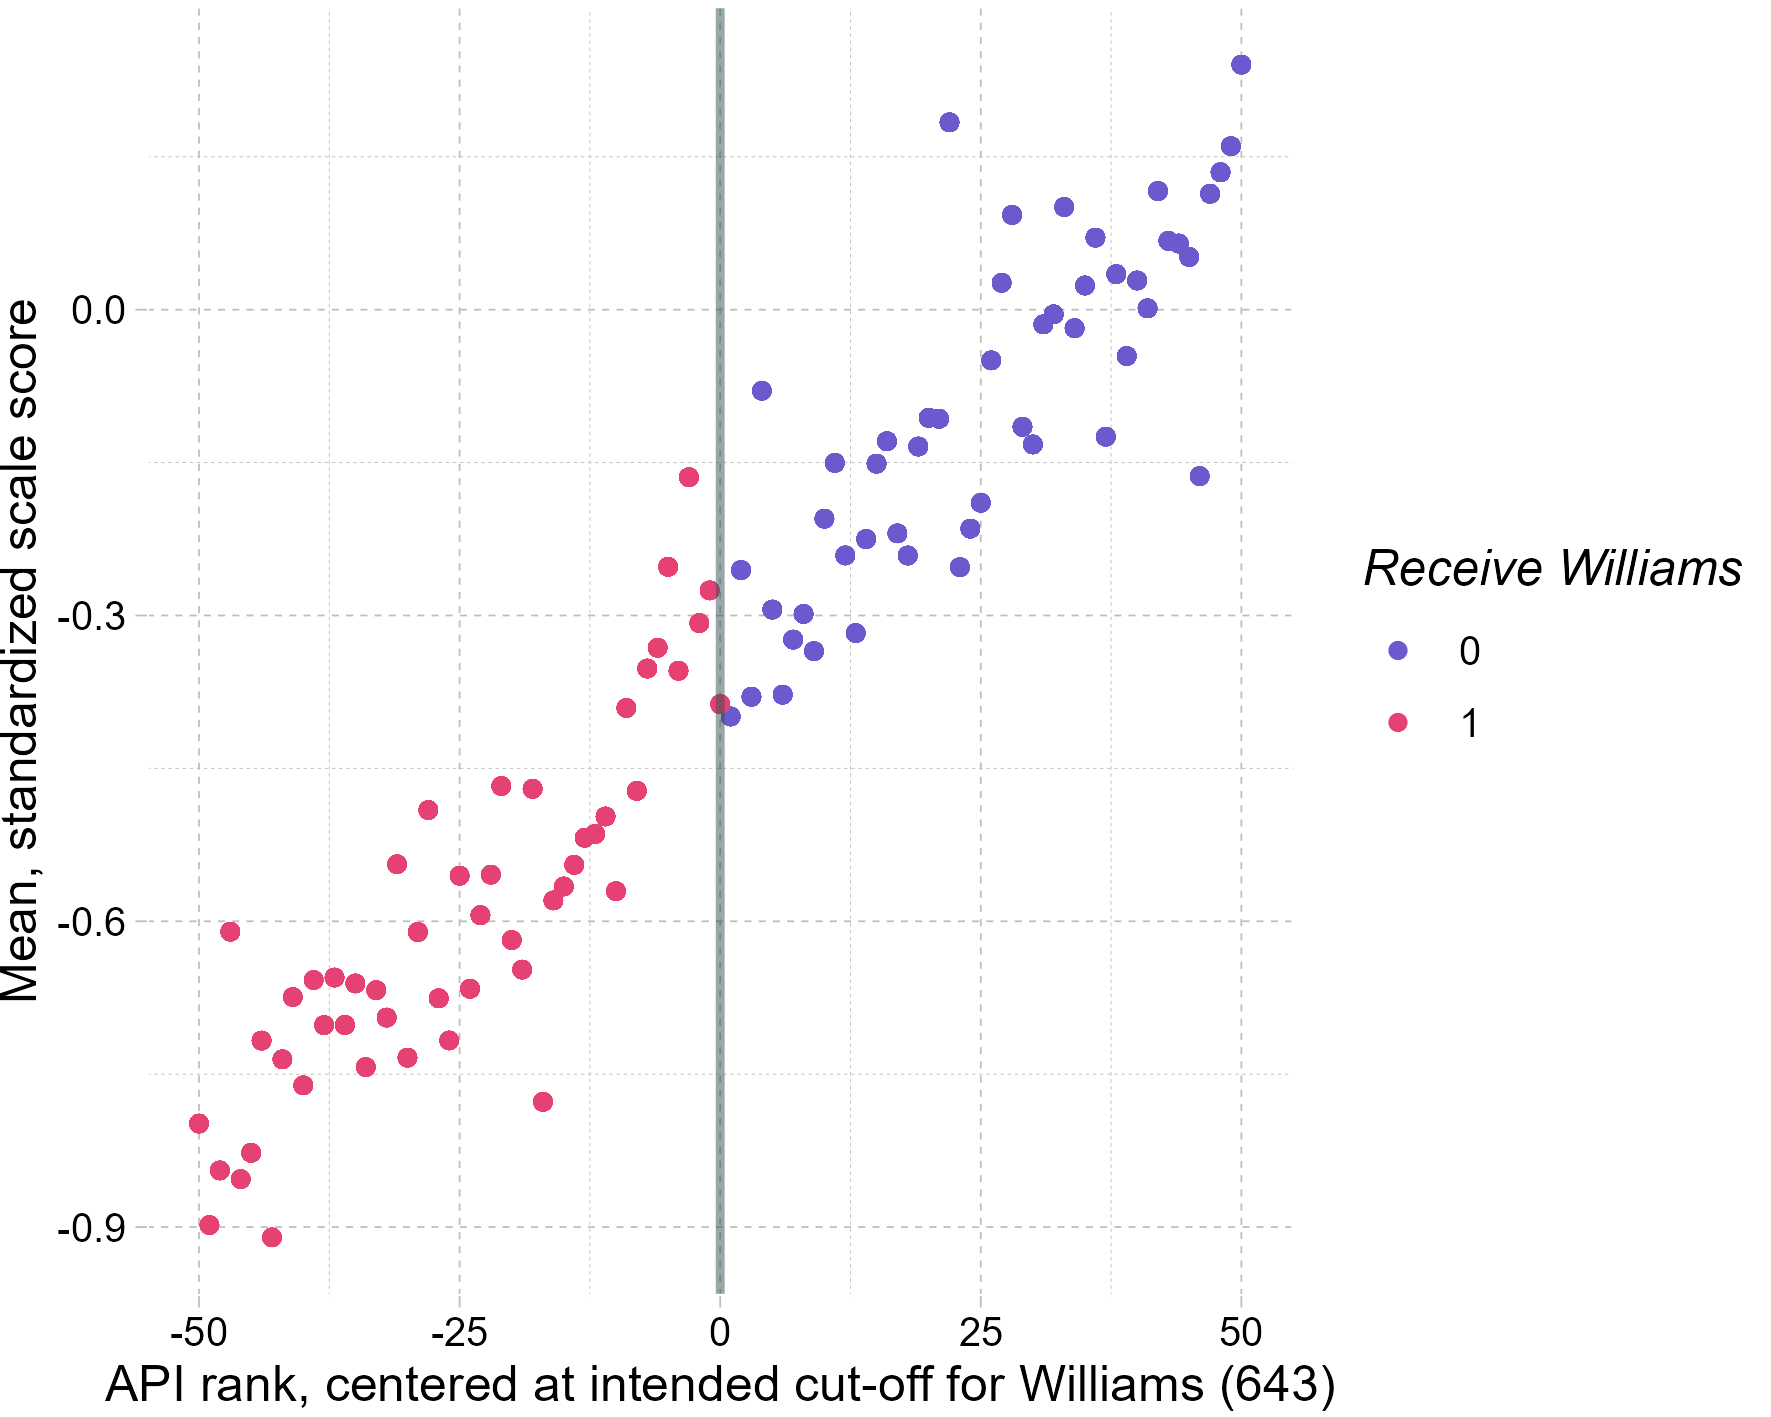
\includegraphics[scale=0.4]{figures/main_RD_effect.png}
}
\subfloat[Binned API values]{
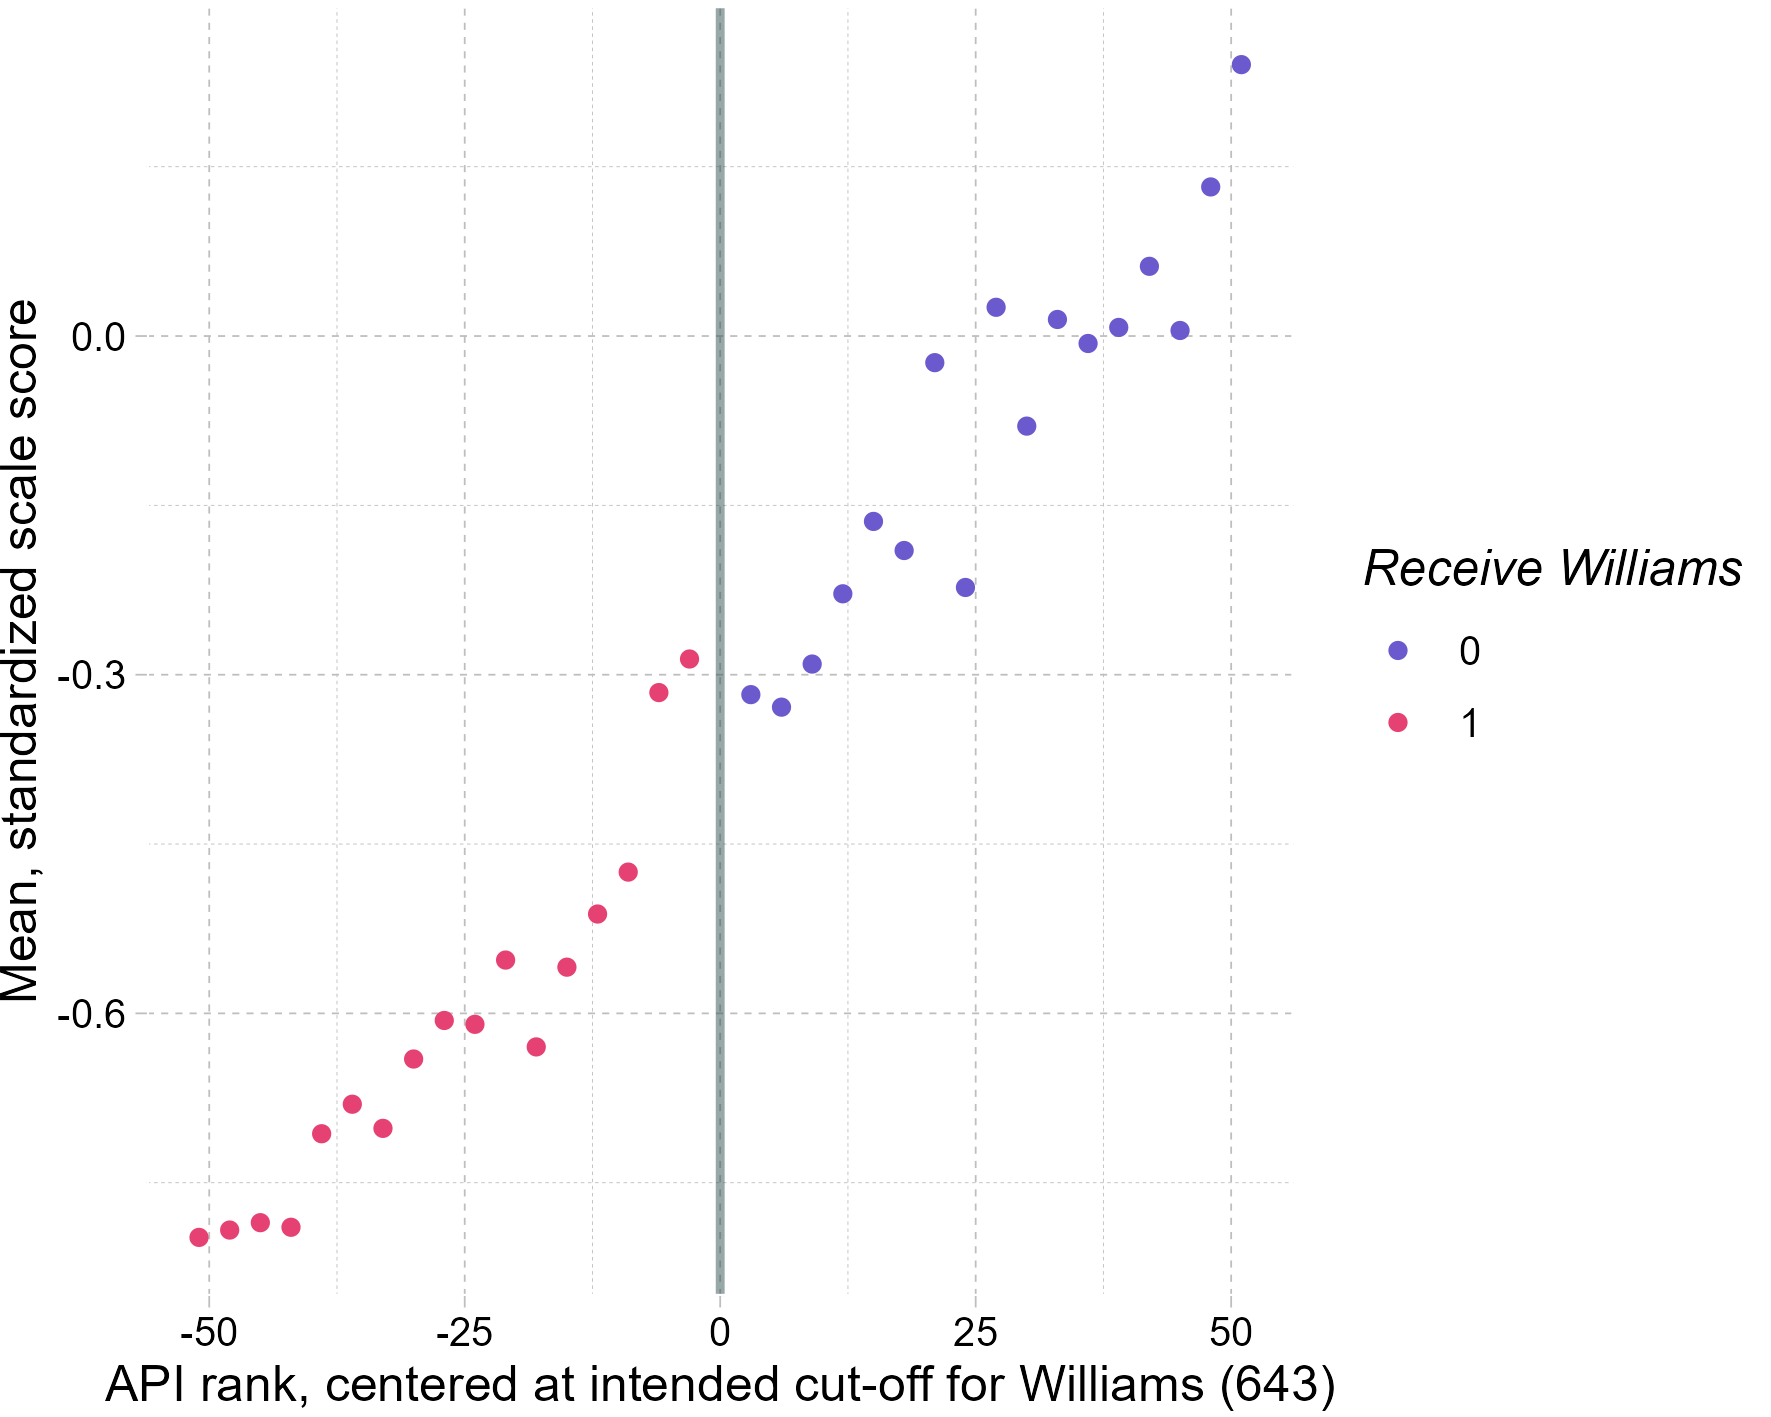
\includegraphics[scale=0.4]{figures/main_RD_effect_bin.png}
}
\caption{Effect of textbook funding on student achievement in elementary schools}
\label{fig:outcome}
\end{center}
\end{figure}


	\item[B2.] We formalize these graphical results by estimating a series of Ordinary Least Squares models in a regression discontinuity framework. Specifically, we estimate:

\begin{equation} 
\begin{aligned}
\text{TESTSCORE}_{it}= & \alpha+ \mathbb{1} \left(APISCORE_{i2003} \leq 643\right)\delta + \\
& f\left(APISCORE_{i2003}\right)+u_{it}
\label{eq:1}
\end{aligned}
\end{equation}

	where $\text{TESTSCORE}_{it}$ is an average of standardized math and reading scores at the school level, the API score (the measure used to allocate differential funding) for elementary school $i$ is measured in 2003. The causal parameter of interest in Equation 1 is the coefficient on the indicator for whether a school was, in fact, eligible for receipt of additional textbook funding ($\delta$). The function $f(\cdot)$ is a flexible, continuous function for which we can vary the functional form and bandwidth.


	In \autoref{tab:rd}, we present a taxonomy of regression discontinuity models of the effect of receipt of textbook funding on test scores.\footnote{Note that these estimates are slightly different from those presented in Holden (2016) as he corrects his standard errors for potential homoskedasticity and weights estimates slightly differently than in standard OLS, though these differences are marginal.}  All models test the effect for school years 2005 to 2009. Models 1, 2 and 4 estimate results in a bandwidth of 19.099 API rank score using the optimal bandwidth selection procedure specified in Calonico, Cattaneo and Titiunik (2014). Model 3 extends the bandwidth to 25 API rank scores. We select the latter range given the evidence that Holden (2016) presents in Figure 8 on the relative stability of coefficient estimates through that bandwidth. Model 1, which imposes a common secular trend on both sides of the discontinuity implies that the receipt of Williams funding improves student test scores by 0.18 school-level standard deviations ($\sigma$). As suggested by graphical evidence, the highest performing schools that receive Williams funding experience the greatest benefit (Model 2). API rank scores are centered on zero and scores below zero are eligible for aid; as a result these coefficients require some interpretation. We predict that schools exactly at the discontinuity (API of 643) will have mean test scores 0.16$\sigma$ higher than those that just exceed the eligibility threshold. We assign schools further from the cutoff negative API scores. Thus the coefficient on the interaction between Williams receipt and API rank reflects how much \textit{less} benefit schools one API score point further away from the discontinuity receive from textbook funding. As an illustrative example, we predict a school with an API score of 638 (centered score of -5) would experience a 0.09$\sigma$ benefit from Williams eligibility ($0.163+0.014 \times (-5)=0.093$).

	Extending the bandwidth to 25 API points in either direction (Model 3) results in somewhat attenuated effects (0.11$\sigma$), but still statistically different than zero and substantively similar in magnitude to our main estimates. Finally, a quadratic specification for the secular trend returns a nearly identical main effect of textbook funding receipt. For reasons of simplicity and completeness, we adopt Model 2 as our preferred specification.


% Table created by stargazer v.5.2.2 by Marek Hlavac, Harvard University. E-mail: hlavac at fas.harvard.edu
% Date and time: Mon, Jan 31, 2022 - 10:02:06 AM
\begin{table}[!htbp] \centering 
  \caption{Regression discontinuity estimates of the effects of instructional material funding on math/reading test scores} 
  \label{tab:rd} 
\begin{tabular}{@{\extracolsep{5pt}}lcccc} 
\hline \hline \\[-1.8ex] 
 & Linear, 		& Linear, 		& Linear 		& Quadratic \\ 
 & same slope 	& diff slope 	& (+/- 25 API) 	&			 \\ 
\\[-1.8ex] & (1) & (2) & (3) & (4)\\ 
\hline \\[-1.8ex] 
 Receive Williams & 0.180$^{***}$ & 0.163$^{***}$ & 0.106$^{**}$ & 0.171$^{***}$ \\ 
  & (0.047) & (0.047) & (0.040) & (0.047) \\ 
  & & & & \\ 
 API Rank & 0.018$^{***}$ & 0.011$^{***}$ & 0.013$^{***}$ & 10.165$^{***}$ \\ 
  & (0.002) & (0.003) & (0.001) & (1.205 \\ 
  & & & & \\ 
 Receive Williams $\times$ &  & 0.014$^{**}$ &  &  \\ 
 API Rank &  & (0.004) &  &  \\ 
  & & & & \\ 
 API Rank sq. &  &  &  & $-$2.007$^{**}$ \\ 
  &  &  &  & (0.618) \\ 
  & & & & \\ 
\hline \\[-1.8ex] 
Observations & 2,680 & 2,680 & 3,510 & 2,680 \\ 
R$^{2}$ & 0.043 & 0.047 & 0.056 & 0.047 \\ 
\hline 
\hline \\[-1.8ex] 
\multicolumn{5}{l}{\textit{Notes:} *p$<$0.05, **p$<$0.01, ***p$<$0.001. Cells report coefficients and assoc-} \\
\multicolumn{5}{l}{iated standard errors. Estimates pool years from 2005 to 2009.} \\ 
\end{tabular} 
\end{table} 


	\item[B3.] Our analysis suggests that increased textbook funding in California between 2005 and 2009 resulted in improved mathematics and reading test scores at the elementary school level. We estimate that schools that were just barely eligible to receive an additional \$96.90 per student in instructional material funding experienced between a 0.10 and 0.18 standard deviation unit improvement in math and reading test scores. 

	\item[B4.] \textbf{\textit{Optional Extension}} Incorporated into B2 above.


\end{enumerate}

\end{document}
